\documentclass[aspectratio=169]{beamer}
\usetheme{focus}

%\usepackage{beamerthemesplit}
%\beamertemplatenavigationsymbolsempty
\usepackage{amsmath}
\usepackage{amsthm}
\usepackage{amssymb}
\usepackage{latexsym}
\usepackage{graphicx}
\usepackage{fancybox}
\usepackage{dsfont}
\usepackage{multirow} 
\usepackage{multicol}
\usepackage{booktabs} 
\usepackage{dcolumn}
\usepackage{soul}
\usepackage[cache=false]{minted}
\usepackage{MnSymbol}
\usepackage{stmaryrd}


\DeclareMathOperator*{\argmax}{arg\,max}
\DeclareMathOperator*{\argmin}{arg\,min}

\newcommand{\X}{\mathtt{X}}
\newcommand{\Y}{\mathtt{Y}}

%\newcommand{\R}{\mathbb{R}}
%\newcommand{\E}{\mathbb{E}}
%\newcommand{\V}{\mathbb{V}}
\newcommand{\p}{\mathbb{P}}
\newcommand*\df{\mathop{}\!\mathrm{d}}
\newcommand{\del}{\partial}


% imports
\usepackage{xargs}
\usepackage{xpatch}
\usepackage{etoolbox}
\usepackage{pdflscape}
\usepackage{booktabs}
\usepackage{threeparttable}
\usepackage[skip=0.2\baselineskip]{caption}

% command for inputting raw latex
\makeatletter
\newcommand\primitiveinput[1]{\@@input #1 }
\makeatother

% common table command
\newcommandx{\tablecontent}[4]{
    \begin{threeparttable}[!ht]
        \centering
        \caption{#3}
        \vspace{-1em}
        \footnotesize
        \begin{tabular}{#1}
            \primitiveinput{../tables/#2.tex}
        \end{tabular}
        \vspace{-0.2em}
        \begin{tablenotes}[flushleft]
            #4
        \end{tablenotes}
    \end{threeparttable}
}




% \usepackage{slashbox}
\title{Lecture 1: Time Series}
\author{Chris Conlon }
\institute{NYU Stern }


\newcommand{\norm}[1]{\left\lVert#1\right\rVert}
\newcommand{\R}{\mathbb{R}}
\newcommand{\E}{\mathbb{E}}
\newcommand{\V}{\mathbb{V}}
\newcommand{\ol}{\overline}
%\newcommand{\ul}{\underline}
\newcommand{\pp}{{\prime \prime}}
\newcommand{\ppp}{{\prime \prime \prime}}
\newcommand{\policy}{\gamma}


\newcommand{\fp}{\frame[plain]}

\date{\today}

\begin{document}
\maketitle

\begin{frame}[fragile]{Packages for Today}
Let's load some packages so that I can make some better looking plots:\\
\begin{minted}{R}
#always
library(tidyverse)
# for loading data
library(tidyquant)
# for cleaning up time series
library(timetk)
library(broom)
library(sweep)
library(forecast)
# for AR regression
library(dynlm)
# for testing
library(ts)
\end{minted}
\end{frame}

\section{What is Time Series?}


\begin{frame}{Big Picture}
So far you have mostly studied \alert{cross sectional econometrics} (subscript $i$):
\begin{itemize}
\item Individual observations are \alert{independent} of one another (mostly).
\item Large number of individuals allows us to do inference (LLN, CLT).
\end{itemize}
\vspace{1cm}
But suppose we observe a single object for may periods (subscript $t$):
\begin{itemize}
\item Now we worry that $y_{t}$ is \alert{autocorrelated} with $y_{t-1}$
\item This means that \alert{independence} is not going to hold.
\item This presents a number of challenges addressed in time series econometrics.
\end{itemize}
\end{frame}

\begin{frame}{Employment}
\begin{center}
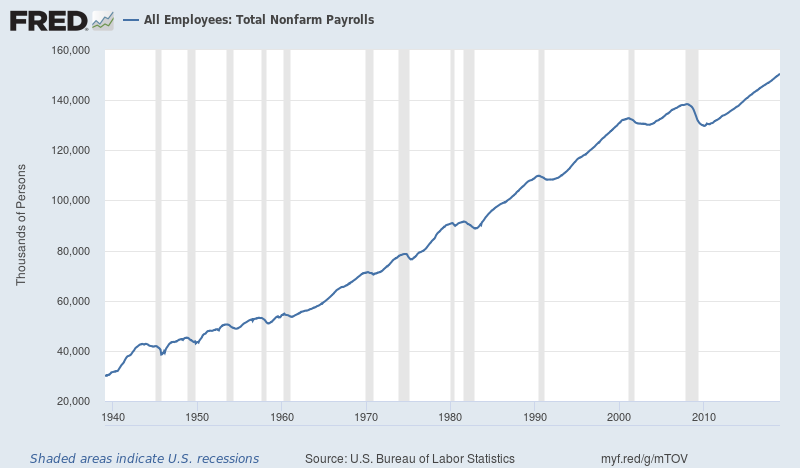
\includegraphics[width=5in]{./resources/nonfarm_level.png}
\end{center}
\end{frame}

\begin{frame}{Employment}
\begin{center}
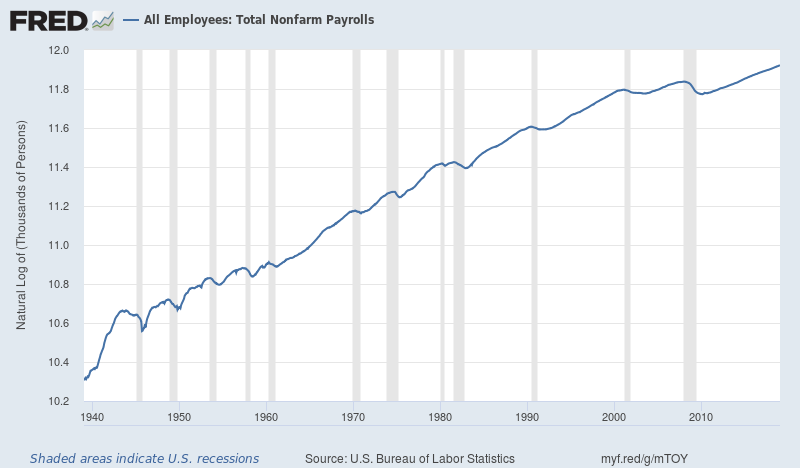
\includegraphics[width=5in]{./resources/nonfarm_log.png}
\end{center}
\end{frame}

\begin{frame}{Employment}
\begin{center}
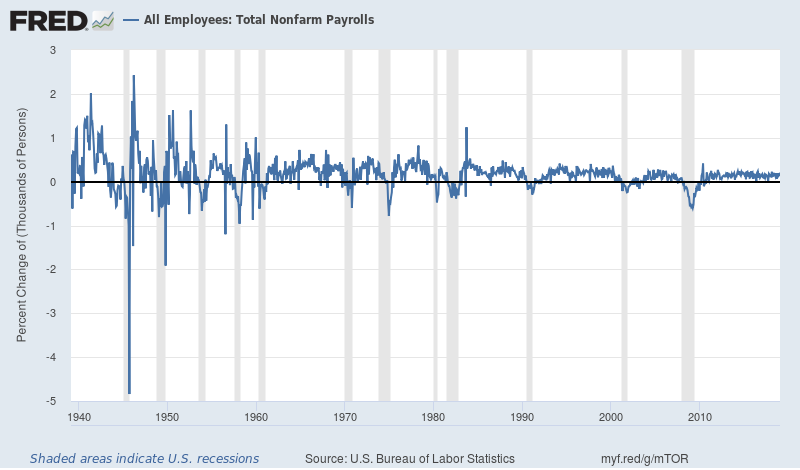
\includegraphics[width=5in]{./resources/nonfarm_pct.png}
\end{center}
\end{frame}

\begin{frame}[fragile]{Do it ourselves}
\begin{minted}{R}
gdp<-tq_get("A191RL1Q225SBEA", get  = "economic.data",
         from='1950-01-1',to='2018-12-31')
tail(gdp)
           A191RL1Q225SBEA
2017-04-01             3.0
2017-07-01             2.8
2017-10-01             2.3
2018-01-01             2.2
2018-04-01             4.2
2018-07-01             3.4
\end{minted}
\end{frame}

\begin{frame}[fragile]{Do it ourselves}
\begin{minted}{R}
ggplot(gdp, aes(date, price)) + geom_line() +
+     scale_x_date() + ylab("Annualized GDP Growth") + xlab("")
\end{minted}
\begin{center}
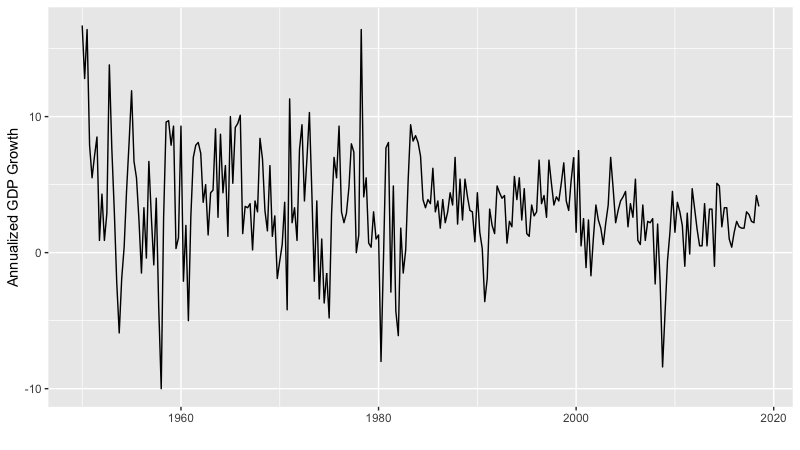
\includegraphics[width=4.5in]{./resources/gdp_plot.png}
\end{center}
\end{frame}





\section{Theory of Time Series}

\begin{frame}{Notation}
We observe a sample $\{y_1,y_2,\ldots,y_{t-1},y_{t},y_{t+1}\}$.
\begin{itemize}
\item We call $y_{y-1}$ the \alert{first lag} of $y_t$.
\item We call $\Delta y_{t} = y_{t} - y_{t-1}$ the \alert{first difference}
\item We might also want $\Delta \ln y_{t} = \ln y_{t} - \ln y_{t-1}$
\item We can approximate percentage change as  $100 \cdot \Delta \ln y_{t}$
\end{itemize}
\end{frame}

\begin{frame}{Autocovariance, Serial Correlation}
Measure the correlation of a series with its own lagged values
\begin{itemize}
\item First \alert{autocovariance} of $y_t$ is $Cov(y_t,y_{t-1}) = \gamma(1)$.
\item The $j$th autocovariance of $y_t$ is $Cov(y_t,y_{t-j})=\gamma(j)$.
\end{itemize}
Questions
\begin{enumerate}
\item How do we represent $Var(y_t)$?
\item Can we show that $\gamma(k) = \gamma(-k)$? (even function)
\item Can we show that $\gamma(0) \geq |\gamma(k)|$ for any $k$?
\item Does this imply that $|\gamma(k)| \geq | \gamma(k-1)|$?
\end{enumerate}
\end{frame}

\begin{frame}{Autocorrelation}
\small
We can also compute the autocorrelaton coefficient $j$: 
\begin{align*}
Corr(y_t,y_{t-j}) = \frac{Cov(y_t,y_{t-j})}{Var(y_t)} = \frac{\gamma(j)}{\gamma(0)} = \rho(j)
\end{align*}
With sample analogue
\begin{align*}
\widehat{Corr(y_t,y_{t-j})} =  \frac{\widehat{\gamma}(j)}{\widehat{\gamma}(0)} = \widehat{\rho}(j)
\end{align*}
Which we can estimate via:
\begin{align*}
\widehat{\rho}(j)=  \frac{1}{T} \sum_{t=j+1}^T(y_t -\overline{y})(y_{t-j} - \overline{y})
\end{align*}
\begin{itemize}
\item Most software uses $\frac{1}{T}$ instead of d.o.f corrected $\frac{1}{T-j}$
\item Some software uses mean of $\{y_{j+1},y_T\}$ and $\{y_{1},y_{T-j}\}$ instead of grand mean
\item Can Correct autocorrelation between $(y_t,y_{t-h})$ removing dependence on $y_1,\ldots , y_{t-h+1}$ [PCF]
\end{itemize}
\end{frame}

\begin{frame}[fragile]{ACF plots}
\begin{center}
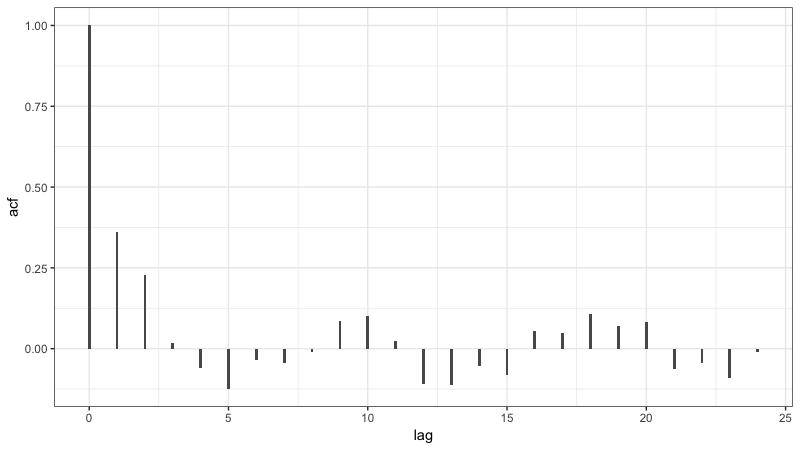
\includegraphics[width=3.5in]{./resources/acf_plot.png}
\end{center}
\begin{minted}{R}
result<-tidy(acf(gdp$price))
ggplot(result, aes(x=lag, y=acf)) +
         geom_bar(stat='identity', width=0.1) + theme_bw()
\end{minted}
\end{frame}


\begin{frame}{Stationarity}
Conceptually \alert{stationarity} is one of the most important issues with time series:
\begin{itemize}
\item Basic idea: the future needs to look like the past (at least probabilistically)
\item I cheated on previous slides and assumed stationarity. Why?
\item Simplified: $Cov(y_t,y_{t-k})$ is allowed to depend on $k$ but not on $t$.
\begin{itemize}
\item Relationship between $y_t$ and its lags is constant across time
\end{itemize}
\item Formally we need the joint distribution $f(y_{s+1},y_{s+2},\ldots,y_{s+T})$ to be invariant to $s$.
\item Weaker form: Covariance Stationary
\end{itemize}
\end{frame}

\begin{frame}{Hand Waving Technical Stuff}
We probably want something like an LLN or CLT:
\begin{itemize}
\item \alert{Independence} is violated between $(y_t,y_{t-k})$
\item Idea: consider a large value $H$ and assume \alert{stationarity}:
\begin{itemize}
\item The block $(y_t,y_{t-1},y_{t-2},\ldots,y_{t-k})$ and $(y_{t+H},y_{t-1+H},y_{t-2+H},\ldots,y_{t-k+H})$ are as if they are independent for some large enough choice of $H$.
\item How is $H$ determined? The \alert{mixing rate} of the time series?
\item In practice? Looking at the ACF function/plot
\end{itemize}
\end{itemize}
\end{frame}

\begin{frame}{Hand Waving Technical Stuff}
\begin{itemize}
\item Soemtimes people will talking about \alert{mixing properties} or the \alert{mixing rate}
\item This tells us how far apart in time two observations are before we can treat them as if they are ``independent''.
\item Another property is \alert{ergodicity}
\begin{align*}
\sum_{k=0}^{\infty} | \gamma(k)|  = \gamma(0) \tau < \infty
\end{align*}
\item $\tau$ is the \alert{correlation} time
\item We could look at the variance of $\overline{X}_t$ to derive this but
\item It is as if we have $\frac{n}{1+ 2\tau}$ \alert{effective independent observations}
\end{itemize}
\end{frame}

\begin{frame}{$AR(1)$ Regression}
Consider the first-order autoregression for a \alert{forecast}:
\begin{align*}
y_t = \beta_0 + \beta_1 Y_{t-1} + \varepsilon_t
\end{align*}
\begin{itemize}
    \item No causal interpretation of $(\beta_0,\beta_1)$.
    \item $\beta_1=0$ means that $y_{t-1}$ is not informative about $y_t$.
    \item We can run this regression using OLS
\end{itemize}
\end{frame}

\begin{frame}{$AR(1)$ Regression}
Consider the first-order autoregression for a \alert{forecast}:
\begin{align*}
y_t = \beta_0 + \beta_1 Y_{t-1} + \varepsilon_t
\end{align*}
\begin{itemize}
    \item No causal interpretation of $(\beta_0,\beta_1)$.
    \item $\beta_1=0$ means that $y_{t-1}$ is not informative about $y_t$.
    \item We can run this regression using OLS
\end{itemize}
\end{frame}


\begin{frame}[fragile]{$AR(1)$ Example}
\begin{minted}{R}
> ar(gdp$price,order=1)

Call:
ar(x = gdp$price, order.max = 1)

Coefficients:
     1  
0.3816  

Order selected 1  sigma^2 estimated as  12.65
\end{minted}
\end{frame}

\begin{frame}{Wold Decomposition}
Start with the AR(1) where $\varepsilon_{t}$ is I.I.D with some variance $\sigma^2$:
\begin{align*}
y_t &= \beta_0 + \beta_1 y_{t-1} + \varepsilon_t\\
y_{t-1} &= \beta_0 + \beta_1 y_{t-2} + \varepsilon_{t-1}\\
y_{t-2} &= \beta_0 + \beta_1 y_{t-3} + \varepsilon_{t-2}
\end{align*}
Can we re-write the sequence as function of $\epsilon_t$'s only?
\begin{align*}
y_t &= \underbrace{\beta_0 + \beta_1 \beta_0 + \beta_1^2 \beta_0}_{\widetilde{\beta}_0} + \beta_1 \varepsilon_{t-1} + \beta_1^2 \varepsilon_{t-2} +  \varepsilon_t \ldots \\
y_t &= \widetilde{\beta}_0 + \sum_{k=1}^{t} \beta^{k} \varepsilon_{t-k}
\end{align*}
\end{frame}


\begin{frame}{Wold Decomposition}
Our $AR(1)$ can be written as a $MA(\infty)$ \alert{moving average process}:
\begin{align*}
y_t &= \widetilde{\beta}_0 + \sum_{k=1}^{\infty} \beta^{k} \varepsilon_{t-k}
\end{align*}
\begin{itemize}
    \item We call this an $MA(\infty)$ process because it represents a $\beta_1$ weighted moving average of \alert{all past realizations} of $\varepsilon_t$
    \item Wold's Theorem tells us we can write any \alert{stationary} time series as the sum of a \alert{deterministc} and \alert{stochastic} component.
\end{itemize}
\end{frame}


\begin{frame}{Wold Decomposition}
Consider the Wold Representation of the $AR(1)$
\begin{align*}
y_t &= \widetilde{\beta}_0 + \sum_{k=1}^{\infty} \beta_1^{k} \varepsilon_{t-k}
\end{align*}
Assume that $\varepsilon \sim N[0,\sigma^2)$ and IID
\begin{align*}
E[y_t] &= \widetilde{\beta}_0 \\
V[y_t] &= \sum_{k=1}^{\infty} \beta_0^{k} Var(\varepsilon_{t-k})  \rightarrow \frac{1}{1-\beta_1} \sigma^2 
\end{align*}
\begin{itemize}
    \item Here \alert{stationarity} requires $\beta_1 \in (0,1)$.
    \item Note that as $\beta_1 \rightarrow 1$ implies that the series no longer converges
    \item This is what is known as a \alert{unit root}
\end{itemize}
\end{frame}

\begin{frame}{Other Autoregressive Processes}
We could also construct an $AR(2)$
\begin{align*}
y_t &= \beta_0 + \beta_1 y_{t-1} + \beta_2 y_{t-2} + \varepsilon_{t}
\end{align*}
Or an $AR(p)$:
\begin{align*}
y_t &= \beta_0 + \sum_{k=1}^p \beta_k y_{t-k} + \varepsilon_{t}
\end{align*}
Or an $ARMA(p,q)$ which adds moving average terms:
\begin{align*}
y_t &= \beta_0 + \sum_{k=1}^p \beta_k y_{t-k} + \sum_{k=1}^p \theta_k \varepsilon_{t-k} 
\end{align*}
\begin{itemize}
\item An important question is \alert{selecting the order of the lag} $p$
\end{itemize}
\end{frame}


\begin{frame}{What About Lag Selection}
Think about the $AR(p)$ model, which order lag do we choose?
\begin{align*}
y_t &= \beta_0 + \sum_{k=1}^p \beta_k y_{t-k} + \varepsilon_{t}
\end{align*}
\begin{itemize}
  \item More lags $\rightarrow$ Better Fit
  \item Potential for \alert{overfitting}
  \item Bias vs. Variance tradeoff
\end{itemize}
\end{frame}

\begin{frame}{Information Criteria}
\begin{align*}
AIC(p) &= \ln \left(\frac{SSR(p)}{T} \right) + (p+1) \frac{2}{T}\\
BIC(p) &= \ln \left(\frac{SSR(p)}{T} \right) + (p+1) \frac{\ln T}{T}
\end{align*}
The penalty is smaller for $AIC$ than for $BIC$
\begin{itemize}
  \item $AIC$ estimates more lags (bigger $p$) than $BIC$
  \item $AIC$ tends to overestimate $p$
\end{itemize}
There are other information criteria and ways to calculate.
\end{frame}

\begin{frame}[fragile]{$AR(p)$ Example: Auto-selecting}
\begin{minted}{R}
> ar(gdp$price)

Call:
ar(x = gdp$price)

Coefficients:
      1        2        3  
 0.3461   0.1505  -0.0880  

Order selected 3  sigma^2 estimated as  12.46
\end{minted}
\end{frame}

\begin{frame}{Autoregressive Distributed Lag Models}
$ADL(p,r)$ models add the covariate $X$ (and its lags). Usually contemporaneous $X_t$ is excluded:
\begin{align*}
y_t &= \beta_0 + \sum_{k=1}^p \beta_k y_{t-k} + \sum_{k=1}^r \theta_k X_{t-k} + \varepsilon_t
\end{align*}
An important issue is \alert{Granger Causality}
\begin{itemize}
\item This has \alert{nothing to do} with actual causality
\item Include $p>r$ lags of $y_t$. Does $(x_t,x_{t-1},\ldots,x_{t-p})$ have any predictive value?
\item Joint F-test of all coefficients on $x_t$ lags
\end{itemize}
\end{frame}

\begin{frame}{Steel Production and Employment}
\begin{center}
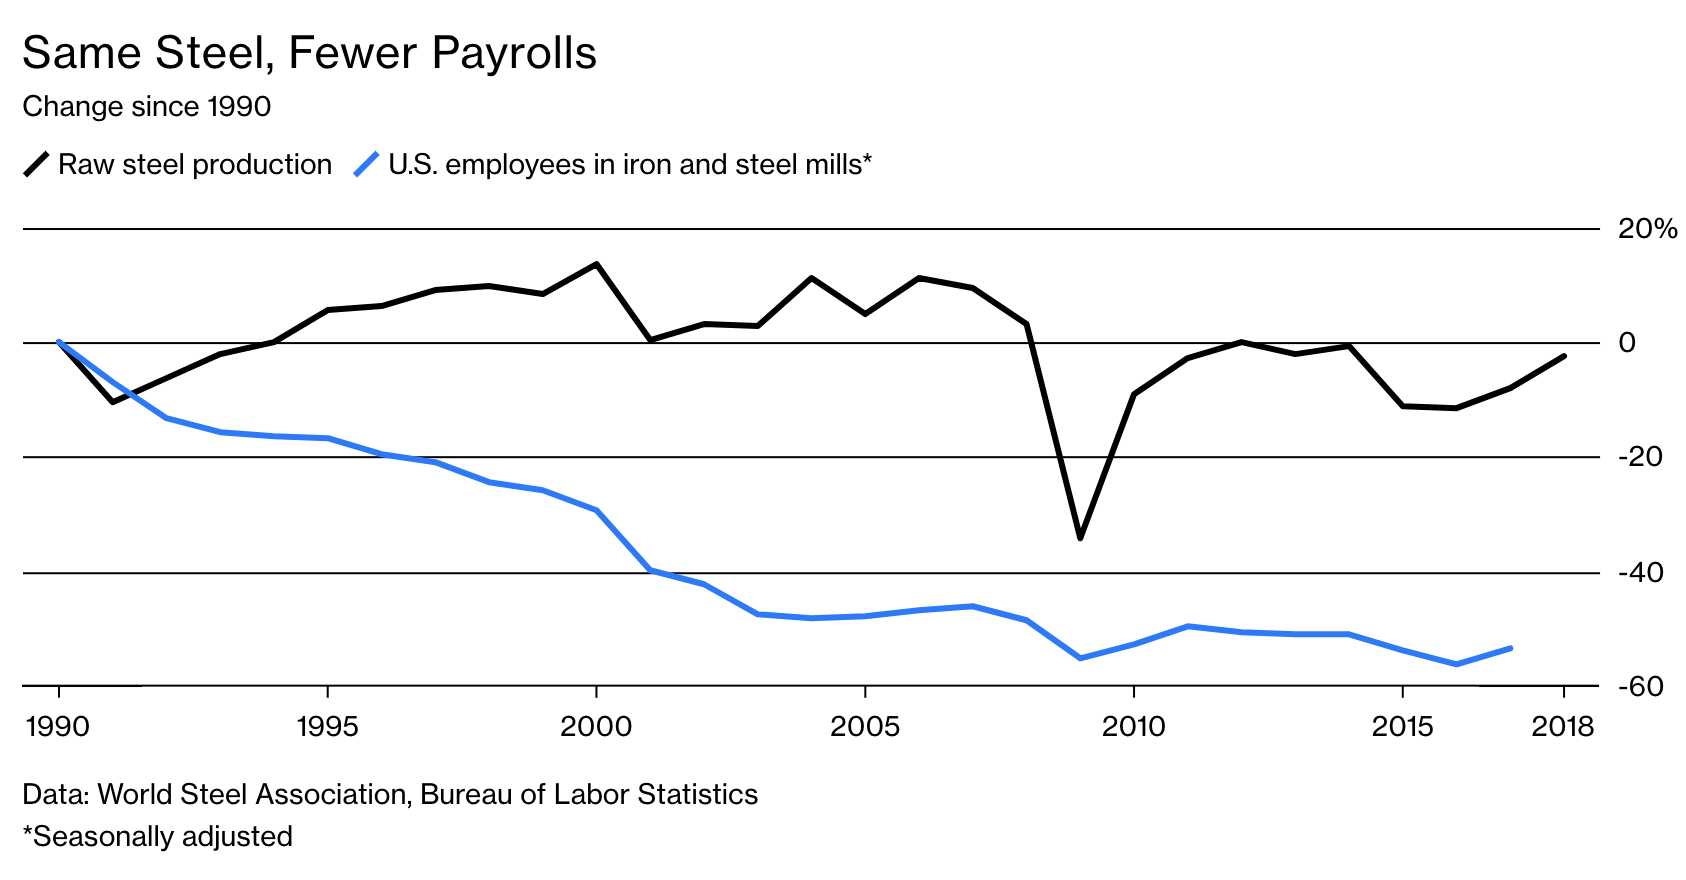
\includegraphics[width=5in]{./resources/steel.png}
\end{center}
\end{frame}

\begin{frame}[fragile]{$ADL(3,3)$ Example}
\tiny
\begin{minted}{R}
dt<-read.csv("steel.csv")
dt2<-ts(dt)
>summary(dynlm(output~L(output,1:3)+L(hours,1:3), data=dt2))

Residuals:
    Min      1Q  Median      3Q     Max 
-34.162  -4.769   0.439   6.952  13.480 

Coefficients:
                 Estimate Std. Error t value Pr(>|t|)   
(Intercept)     196.56293   55.49461   3.542  0.00205 **
L(output, 1:3)1  -0.01371    0.29492  -0.046  0.96339   
L(output, 1:3)2   0.01829    0.31067   0.059  0.95363   
L(output, 1:3)3  -0.17356    0.21767  -0.797  0.43459   
L(hours, 1:3)1    0.46844    0.92788   0.505  0.61918   
L(hours, 1:3)2   -0.90532    1.33926  -0.676  0.50679   
L(hours, 1:3)3   -0.20820    0.84409  -0.247  0.80769   
---
Signif. codes:  0 ?***? 0.001 ?**? 0.01 ?*? 0.05 ?.? 0.1 ? ? 1

Residual standard error: 10.44 on 20 degrees of freedom
Multiple R-squared:  0.5985,	Adjusted R-squared:  0.478 
F-statistic: 4.969 on 6 and 20 DF,  p-value: 0.002905
\end{minted}

\end{frame}


\begin{frame}[fragile]{Granger Test}
\begin{minted}{R}
>grangertest(output~ hours, order=3,data=dt)
Granger causality test

Model 1: output ~ Lags(output, 1:3) + Lags(hours, 1:3)
Model 2: output ~ Lags(output, 1:3)
  Res.Df Df      F  Pr(>F)  
1     20                    
2     23 -3 3.8094 0.02612 *
---
Signif. codes:  0 ?***? 0.001 ?**? 0.01 ?*? 0.05 ?.? 0.1 ? ? 1
\end{minted}
Significant! Hours predict output.
\end{frame}

\begin{frame}[fragile]{Granger Test: Other Direction}
\begin{minted}{R}
> grangertest(hours ~ output, order=3,data=dt)
Granger causality test

Model 1: hours ~ Lags(hours, 1:3) + Lags(output, 1:3)
Model 2: hours ~ Lags(hours, 1:3)
  Res.Df Df      F Pr(>F)
1     20                 
2     23 -3 1.8272 0.1747
\end{minted}
Not significant! Output does not predict hours.
\end{frame}

\section{Trends}

\begin{frame}{Which Series has a Trend?}
\begin{center}
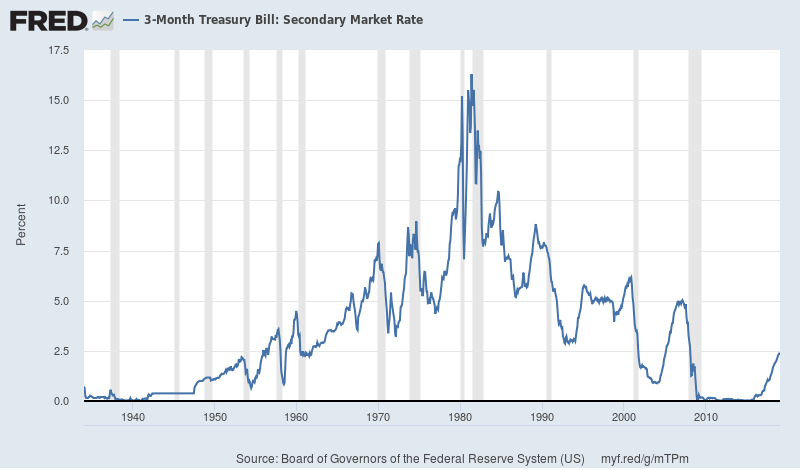
\includegraphics[width=5in]{./resources/treasury_90.png}
\end{center}
\end{frame}

\begin{frame}{Which Series has a Trend?}
\begin{center}
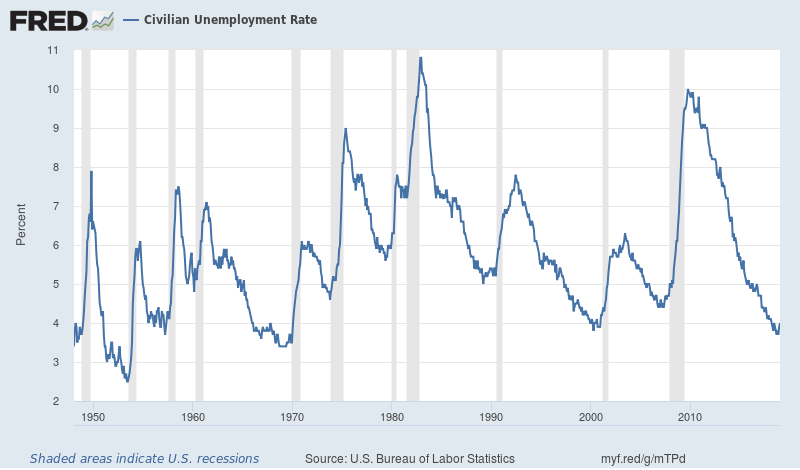
\includegraphics[width=5in]{./resources/unemployment.png}
\end{center}
\end{frame}

\begin{frame}{Which Series has a Trend?}
\begin{center}
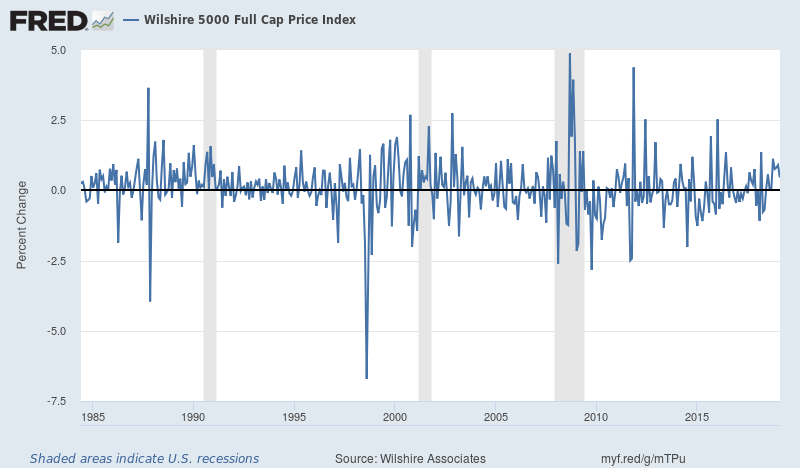
\includegraphics[width=5in]{./resources/wilshire_5000.png}
\end{center}
\end{frame}

\begin{frame}{Two Kinds of Trends}
\begin{itemize}
\item Deterministic Trends: $y_t = a\cdot t + \epsilon_t$ or $y_t = a\cdot t + b \cdot t^2 + \epsilon_t$
\item Stochastic Trend: random and time varying trend (see how this works later)
\item Random Walk: $Y_t = Y_{t-1} + \varepsilon_t$
\end{itemize}
\end{frame}

\begin{frame}{What is a random walk}
\begin{align*}
Y_t = Y_{t-1} + \varepsilon_t, \quad E[\varepsilon_t] = 0, V[\varepsilon_t] = \sigma^2
\end{align*}
\begin{itemize}
\item Best guess of tomorrow is today
\item $E[y_{t+h} | y_t] = y_t$ for any $t$ and $h$
\item If $Y_0$ then $V(y_t) = t \sigma^2$
\end{itemize}
\end{frame}


\begin{frame}[fragile]{Generate Random Random Walks}
\begin{minted}{R}
tibble(x = 1:1000, y = cumsum(rnorm(1000, mean = 0))) %>% 
  ggplot(aes(x=x,y=y))+
  geom_point()+
  geom_line()
\end{minted}
\end{frame}

\begin{frame}{Adding Drift}
We an easily add a drift term $\beta_0$
\begin{align*}
Y_t = Y_{t-1} + \beta_0 + \varepsilon_t
\end{align*}
\begin{itemize}
\item $E[y_{t+h} | y_t] = y_t + h\cdot \beta_0$ for any $t$ and $h$
\item If $Y_0$ then $V(y_t) = t \sigma^2$
\end{itemize}
Log stock prices are roughly RWD\\
(stock returns are random but positive on average)
\end{frame}

\begin{frame}{Where are we heading?}
Suppose we have a stochastic (random walk) trend:
\begin{itemize}
\item We no longer satisfy \alert{stationarity}
\item We can run OLS but we can't trust the results (not even a little bit)
\begin{itemize}
    \item Recall $AR(1)$ has non-convergent series!
    \item Coefficients are biased towards zero
    \item Not asymptotically normal
\end{itemize}
\item We are going to want to transform things to return to stationary case
\item Easy for RW trend because $\Delta y_t$ is stationary!
\end{itemize}
\begin{align*}
y_t &= y_{t-1} + \varepsilon_t \\
\Delta y_t &= \varepsilon_t
\end{align*}
\end{frame}


\begin{frame}{A Simple Example: $AR(1)$}
We can think about RWD as a special case of $AR(1)$ with $\beta_1=1$
\begin{align*}
Y_t  &= \beta_0 +\beta_1 Y_{t-1} + \varepsilon_t \quad AR(1)\\
Y_t  &= \beta_0 + Y_{t-1} + \varepsilon_t \quad  \text{RWD} \\
\Delta Y_t  &= \beta_0 + \varepsilon_t 
\end{align*}
We call the $\beta_1$ case \alert{unit root} because $1 - \beta_1 z=0$ has root $z = \frac{1}{\beta_1}$ so that $\beta_1$ when $z=1$.
\end{frame}

\begin{frame}{Harder Example: $AR(2)$}
This case is more complicated
\begin{align*}
Y_t &= \beta_0 + \beta_1 Y_{t-1} + \beta_2 Y_{t-2} + \varepsilon_t\\
    &= \beta_0 + (\beta_1 + \beta_2) Y_{t-1} - \beta_2 Y_{t-1} +  \beta_2 Y_{t-2} + \varepsilon_t\\
    &= \beta_0 + (\beta_1 + \beta_2) Y_{t-1} - \beta_2(Y_{t-1} - Y_{t-2})+ \varepsilon_t\\
\end{align*}
Now difference $Y_{t-1}$:
\begin{align*}
Y_t -Y_{t-1}&= \beta_0 + \underbrace{(\beta_1 + \beta_2 -1)}_{\delta} Y_{t-1} - \beta_2 \underbrace{(Y_{t-1} - Y_{t-2})}_{\Delta Y_t}+ \varepsilon_t\\
\Delta Y_t &= \beta_0 + \delta Y_{t-1} - \beta_2 \Delta Y_t  \varepsilon_t\\
\end{align*}
\end{frame}



\begin{frame}{A Harder Example: $AR(2)$}
What is a unit root now?
\begin{align*}
\Delta Y_t &= \beta_0 + \delta Y_{t-1} - \beta_2 \Delta Y_t  \varepsilon_t
\end{align*}
\begin{itemize}
\item $1- \beta_1 z - \beta_2 z^2 = 0$ a unit root implies that $\beta_1 + \beta_2=1$
\item If there is a unit root then $\delta=0$
\begin{itemize}
\item We can use this to construct a test for a unit root
\end{itemize}
\item If $AR(2)$ has a unit root, then write as an $AR(1)$ in first differences
\end{itemize}
\begin{align*}
\Delta Y_t &= \beta_0 - \beta_2 \Delta Y_t  \varepsilon_t\\
\end{align*}
\end{frame}

\begin{frame}{The General Case $AR(p)$}
What is a unit root now?
\begin{align*}
Y_t &= \beta_0 + \beta_1 Y_{t-1} + \beta_2 Y_{t-2} + \cdot + \beta_p Y_{t-p} + \varepsilon_t\\
\Delta Y_t &= \beta_0 + \Delta Y_{t-1} + \gamma_1 \Delta Y_{t-1} + \gamma_2 \Delta Y_{t-2} +  \cdots +  \gamma_p \Delta Y_{t-p}  + \varepsilon_t
\end{align*}
With coefficients:
\begin{align*}
\delta &= \beta_1 + \beta_2 + \cdots + \beta_p -1\\
\gamma_1 &=  -(\beta_2 + \cdots + \beta_p)\\
\gamma_2 &=  -(\beta_3 + \cdots + \beta_p)\\
\gamma_{p-1} &=  -\beta_p
\end{align*}
\begin{itemize}
    \item Thus the $AR(p)$ becomes an $AR(p-1)$ in first differences.
    \item Again $\delta=0$ tells us whether or not unit root is present
\end{itemize}
\end{frame}

\begin{frame}{Detecting Trends}
\begin{itemize}
\item Plot the Data: are there persistent long run movements?
\item Run the Dickey-Fuller Test for unit roots
\end{itemize}
Dickey Fuller Test for $AR(1)$:
\begin{align*}
Y_t &= \beta_0 + \beta_1 Y_{t_1} +\varepsilon_t\\
\Delta Y_t &= \beta_0 + \delta Y_{t-1} + \mu \cdot t + \varepsilon_t
\end{align*}
\begin{itemize}
\item $H_0: \delta = 0$ vs $H_1: \delta < 0$ (one sided test)
\item The usual critical values for t-stats don't work (because at $\delta=0$ things are non-normal).
\item Software usually has adjusted critical values
\end{itemize}
\end{frame}


\begin{frame}{Dickey Fuller Test}
Which test do we want?
\begin{align*}
\Delta Y_t &= \beta_0 + \delta Y_{t-1} + \mu \cdot t + \varepsilon_t
\end{align*}
\begin{itemize}
\item Can include the trend $\mu \cdot t$ or not
\item Leads to different critical values
\item Depends on whether $y_t$ is stationary around a trend or not
\item Need to choose number of lags first
\end{itemize}
\end{frame}


\begin{frame}[fragile]{Dickey Fuller Test: Example}
\small
\begin{minted}{R}
# convert to time-series
gdp2<-ts(gdp$price)
> tidy(dynlm(d(gdp2)~L(gdp2,1)+L(d(gdp2),2:4)))
# A tibble: 5 x 5
  term             estimate std.error statistic  p.value
  <chr>               <dbl>     <dbl>     <dbl>    <dbl>
1 (Intercept)        2.19      0.280       7.80 1.40e-13
2 L(gdp2, 1)        -0.693     0.0593    -11.7  9.98e-26
3 L(d(gdp2), 2:4)2   0.128     0.0553      2.32 2.12e- 2
4 L(d(gdp2), 2:4)3   0.0786    0.0609      1.29 1.98e- 1
5 L(d(gdp2), 2:4)4   0.0683    0.0547      1.25 2.12e- 1
\end{minted}
\end{frame}


\begin{frame}[fragile]{Dickey Fuller Test: Example}
\small
\begin{minted}{R}
adf.test(gdp2, k=3)

    Augmented Dickey-Fuller Test

data:  gdp2
Dickey-Fuller = -8.1364, Lag order = 3, p-value = 0.01
alternative hypothesis: stationary
\end{minted}
\end{frame}


\begin{frame}{Spurious Regression/Correlation}
Imagine we have two series each with a trend
\begin{align*}
y_{t} &= a_0 + a_1 t + \varepsilon_{t}\\
x_{t} &= b_0 + b_1 t + \mu_{t}
\end{align*}
\begin{itemize}
    \item Both are related to $t$ but neither has anything to do with each other.
    \item Regression of $x_t$ on $y_t$ can produce very high $R^2$
\end{itemize}
\begin{align*}
y_{t} &= \beta_0  + \beta_1 x_{t} + \varepsilon_t\\
y_{t} &= \beta_0  + \beta_1 (b_0 + b_1 \cdot t + \mu_t) + \varepsilon_t\\
y_{t} &= \underbrace{(\beta_0  + \beta_1 b_0)}_{\widetilde{\beta}_0}  + \underbrace{\beta_1 b_1}_{\widetilde{\beta}_1} \cdot t + \underbrace{(\beta_1 \mu_t+ \varepsilon_t)}_{\widetilde{\varepsilon}_t}\\
\end{align*}
\end{frame}

\begin{frame}{Spurious Regression/Correlation}
\begin{itemize}
\item This is a \alert{huge mistake} and people make it all of the time
\item \url{http://www.tylervigen.com/spurious-correlations}
\item This problem is insidious: it seems obvious and then you do it
\end{itemize}
\end{frame}


\section{Applications of Time Series}

\begin{frame}{Moving Average Models}
 We might want a \alert{trend} but one that isn't a straight line.\\ Enter the simple $q$ Moving average (SMA):
\begin{align*}
Y_t &= \frac{Y_{t-1}+ Y_{t-2} + \cdot + Y_{t-m}}{m}
\end{align*}
\begin{itemize}
\item The average \alert{age} of the data is around $\frac{m+1}{2}$ periods.
\item We are always behind what is happening at time $t$
\item As we include more lags, we use more data, but we get further behind today.
\item Gets plotted a lot on stock market prices, etc.
\end{itemize}
\end{frame}

\begin{frame}{Moving Average: S\&P 500 w/ MA(60)}
\begin{center}
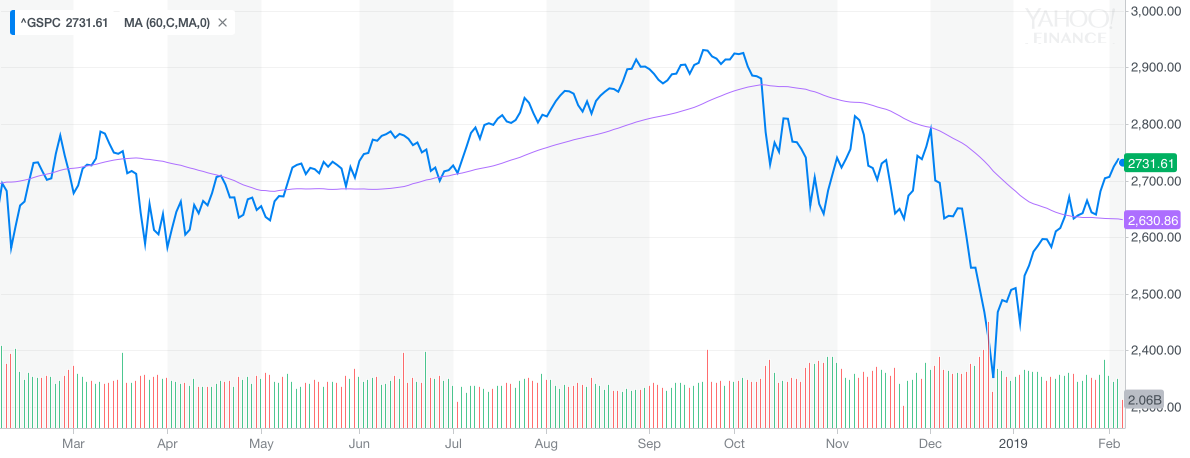
\includegraphics[width=5.5in]{./resources/sp-chart.png}
\end{center}
\end{frame}

\begin{frame}{Simple Exponential Smoothing (SES)}
We might want to weight older observations less and more recent observations more. Think about $L_t=E[Y_{t+1}|Y_t]$ our forecast of $Y_{t+1}$:
\begin{align*}
L_t = \alpha Y_t + (1-\alpha) L_{t-1}\\
E[Y_{t+1}|Y_t]] = \alpha Y_t + (1-\alpha) \hat{Y}_{t}
\end{align*}
Notice that $\varepsilon_t \equiv Y_t - E[Y_t| Y_{t_1}]$ so that
\begin{align*}
E[Y_{t+1}|Y_t]] = \alpha E[Y_t| Y_{t-1}] + \alpha \varepsilon_t
\end{align*}
Rewriting as a \alert{moving average}
\begin{align*}
E[Y_{y+1} | Y_t] = \alpha [ Y_t + (1-\alpha)Y_{t-1} + (1-\alpha)^2 Y_{t-2} + (1-\alpha)^3 Y_{t-3} + \ldots]
\end{align*}
\begin{itemize}
    \item Update the old forecast in direction of forecast error
    \item $\alpha=0$ constant, $\alpha=1$ RW
\end{itemize}
\end{frame}


\begin{frame}{Decomposing Trends and Seasonality}
Given some time series data how should we start?
\begin{itemize}
\item Plot the series
\item Try and \texttt{decompose} the series
\begin{itemize}
\item Extract \alert{trends}
\item Look for \alert{seasonality}
\item Remainder should be \alert{random}
\end{itemize}
\end{itemize}
\end{frame}

\begin{frame}[fragile]{Loading Alcohol Data : }
\small
\url{https://fred.stlouisfed.org/series/S4248SM144NCEN}
\begin{minted}{R}
alcohol_sales_tbl <- tq_get("S4248SM144NCEN", 
                            get  = "economic.data", 
                            from = "2007-01-01",to   = "2016-12-31")
                           # A tibble: 120 x 2
   date       price # note expenditure not prices!
   <date>     <int>
 1 2007-01-01  6627
 2 2007-02-01  6743
 3 2007-03-01  8195
 4 2007-04-01  7828
 5 2007-05-01  9570
 6 2007-06-01  9484
 7 2007-07-01  8608
 8 2007-08-01  9543
 9 2007-09-01  8123
10 2007-10-01  9649
# ? with 110 more rows
\end{minted}
\end{frame}

\begin{frame}[fragile]{Plotting Alcohol Data}
\small
\begin{minted}{R}
alcohol_sales_tbl %>%
    ggplot(aes(x = date, y = price)) +
    geom_line(size = 1, color = palette_light()[[1]]) +
    geom_smooth(method = "loess") +
    labs(title = "US Alcohol Sales: Monthly", x = "", y = "Millions") +
    scale_y_continuous(labels = scales::dollar) +
    scale_x_date(date_breaks = "1 year", date_labels = "%Y") +
    theme_tq()
\end{minted}
\end{frame}

\begin{frame}{Alcohol Example}
\begin{center}
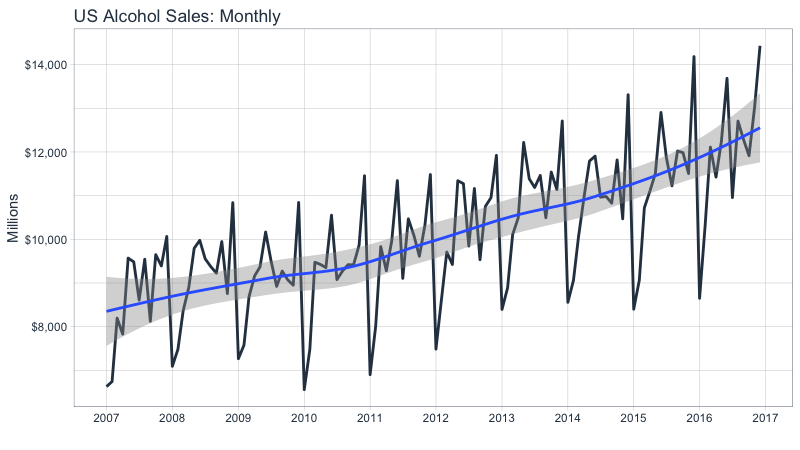
\includegraphics[width=5in]{./resources/alcohol.png}
\end{center}
\end{frame}


\begin{frame}[fragile]{Rearranging Alcohol Data}
Notice the strong seasonal pattern (December and June)
\footnotesize
\begin{minted}{R}
> alcohol_sales_ts <- tk_ts(alcohol_sales_tbl, start = 2007, 
				freq = 12, silent = TRUE)
> alcohol_sales_ts
       Jan   Feb   Mar   Apr   May   Jun   Jul   Aug   Sep   Oct   Nov   Dec
2007  6627  6743  8195  7828  9570  9484  8608  9543  8123  9649  9390 10065
2008  7093  7483  8365  8895  9794  9977  9553  9375  9225  9948  8758 10839
2009  7266  7578  8688  9162  9369 10167  9507  8923  9272  9075  8949 10843
2010  6558  7481  9475  9424  9351 10552  9077  9273  9420  9413  9866 11455
2011  6901  8014  9832  9281  9967 11344  9106 10469 10085  9612 10328 11483
2012  7486  8641  9709  9423 11342 11274  9845 11163  9532 10754 10953 11922
2013  8395  8888 10110 10493 12218 11385 11186 11462 10494 11540 11138 12709
2014  8557  9059 10055 10977 11792 11904 10965 10981 10828 11817 10470 13310
2015  8400  9062 10722 11107 11508 12904 11869 11224 12022 11983 11506 14183
2016  8650 10323 12110 11424 12243 13686 10956 12706 12279 11914 13025 14431
\end{minted}
\end{frame}

\begin{frame}[fragile]{Rearranging Alcohol Data}
Apply \alert{Error Trend Seasonal} Decomposition (ETS) to data. These are not really interpretable on their own:
\tiny
\begin{minted}{R}
> fit_ets <- alcohol_sales_ts %>%
+     ets()
ETS(M,Ad,M) 

Call:
 ets(y = .) 

  Smoothing parameters:
    alpha = 0.0783 
    beta  = 0.0772 
    gamma = 0.0053 
    phi   = 0.9511 

  Initial states:
    l = 8387.3061 
    b = 39.5634 
    s = 1.1755 1.0241 1.041 0.9894 1.0455 0.9968
           1.1104 1.0675 0.9733 0.9743 0.8323 0.7699

  sigma:  0.0451

     AIC     AICc      BIC 
2058.006 2064.778 2108.181 
\end{minted}
\end{frame}


\begin{frame}[fragile]{Rearranging Alcohol Data}
Run the equivalent of \texttt{decompose} on the data:
\footnotesize
\begin{minted}{R}
> decomp_fit_ets <- sw_tidy_decomp(fit_ets)
> decomp_fit_ets 
# A tibble: 121 x 5
   index         observed level slope season
   <S3: yearmon>    <dbl> <dbl> <dbl>  <dbl>
 1 Dec 2006            NA 8387.  39.6  1.18 
 2 Jan 2007          6627 8439.  51.7  0.770
 3 Feb 2007          6743 8458.  19.4  0.832
 4 Mar 2007          8195 8471.  13.4  0.974
 5 Apr 2007          7828 8450. -21.3  0.973
 6 May 2007          9570 8471.  21.1  1.07 
 7 Jun 2007          9484 8495.  23.9  1.11 
 8 Jul 2007          8608 8527.  31.8  0.997
 9 Aug 2007          9543 8602.  74.2  1.05 
10 Sep 2007          8123 8636.  34.9  0.989
\end{minted}
\end{frame}



\begin{frame}{ETS/\texttt{decompose} Example}
\begin{center}
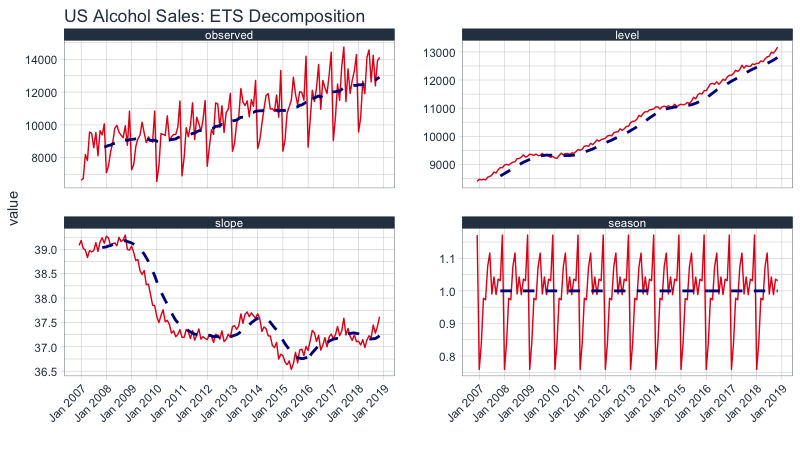
\includegraphics[width=5in]{./resources/ets_decomp.png}
\end{center}

\end{frame}

\begin{frame}{ARIMA Models}
Consider \alert{Auto-Regressive Integrated Moving Average} $ARIMA(p,d,q)$
\begin{itemize}
\item \alert{Autoregressive} $p$ terms like $AR(p)$: lags of $y_{t-p}$
\item \alert{Integrated} $d$ Differenced out unit roots 
\item \alert{Moving Average} $q$ include lags of forecast errors $\epsilon_{t-h}$
\end{itemize}
\end{frame}

\begin{frame}{ARIMA Models}
Denote by $(p,d,q$)
\begin{itemize}
\item $(0,0,0) + c$ constant model
\item $(0,1,0)$ RW
\item $(0,1,0)+ c$ RW w/ drift
\item $(1,0,0)$ $y_t \sim y_{t-1}$
\item $(1,1,0)$ $\Delta y_t \sim \Delta y_{t-1}$
\item $(2,1,0)$ $\Delta y_t \sim \Delta y_{t-1}+\Delta y_{t-2}$
\item $(0,1,1)$ SES model
\item $(0,1,1)+c$ SES with constant trend
\end{itemize}
\end{frame}



\begin{frame}{More Serious: X-13 ARIMA}
Lots of government economic series are \alert{seasonally adjusted}
\begin{itemize} 
\item The Census uses X-13 software to seasonally adjust most series
\item Also popular is Bank of Spain (SEATS) adjustment
\item available in R package \texttt{seasonal}
\item \url{https://github.com/christophsax/seasonal/wiki/Examples-of-X-13ARIMA-SEATS-in-R}
\end{itemize}
\end{frame}


\begin{frame}{Next time: Panel Data}
\begin{itemize} 
\item Linear Model
\item Serial Correlation
\item Fixed Effects, Random Effects
\item Dynamic Panel: Arellano Bond, etc.
\end{itemize}
\end{frame}






\section*{Thanks!}

\end{document}